%------------------------
% Resume Template
% Author : Montasim
% Github : https://github.com/montasim
% License : MIT
%------------------------

\documentclass[a4paper]{article}

\usepackage{latexsym}
\usepackage[empty]{fullpage}
\usepackage{titlesec}
\usepackage{marvosym}
\usepackage{color}
\usepackage{verbatim}
\usepackage{enumitem}
\usepackage{hyperref}
\usepackage{fancyhdr}
\usepackage{lastpage}
\usepackage{graphicx}
\graphicspath{ {./} }

\pagestyle{fancy}
\fancyhf{} % clear all header and footer fields
\fancyfoot{}
\renewcommand{\headrulewidth}{0pt}
\renewcommand{\footrulewidth}{0pt}

% Adjust margins
\addtolength{\oddsidemargin}{-0.530in}
\addtolength{\evensidemargin}{-0.375in}
\addtolength{\textwidth}{1in}
\addtolength{\topmargin}{-.45in}
\addtolength{\textheight}{1in}

\urlstyle{rm}

\raggedbottom
\raggedright
\setlength{\tabcolsep}{0in}

% Sections formatting
\titleformat{\section}{
  \vspace{-10pt}\scshape\raggedright\large
}{}{0em}{}[\color{black}\titlerule \vspace{-6pt}]

%-------------------------
% Custom commands
\newcommand{\resumeItem}[2]{
  \item\small{
    \textbf{#1}{: #2 \vspace{-2pt}}
  }
}

\newcommand{\resumeItemWithoutTitle}[1]{
  \item\small{
    {\vspace{-2pt}}
  }
}

\newcommand{\resumeSubheading}[4]{
  \vspace{-1pt}\item
    \begin{tabular*}{0.97\textwidth}{l@{\extracolsep{\fill}}r}
      \textbf{#1} & #2 \\
      \textit{#3} & \textit{#4} \\
    \end{tabular*}\vspace{-5pt}
}


\newcommand{\resumeSubItem}[2]{\resumeItem{#1}{#2}\vspace{-3pt}}

\renewcommand{\labelitemii}{$\circ$}

\newcommand{\resumeSubHeadingListStart}{\begin{itemize}[leftmargin=*]}
\newcommand{\resumeSubHeadingListEnd}{\end{itemize}}
\newcommand{\resumeItemListStart}{\begin{itemize}}
\newcommand{\resumeItemListEnd}{\end{itemize}\vspace{-5pt}}



%------------------------------ CV STARTS HERE ---------------------------------
\begin{document}
\rfoot{Page \thepage \hspace{2pt} of \hspace{2pt}\pageref{LastPage}}





%------------------------------START HEADING------------------------------------
\begin{tabular*}{\textwidth}{l@{\extracolsep{\fill}}r}
  \textbf{{\LARGE Mohammad Montasim -Al- Mamun Shuvo}} \\
  \textbf{{Developer and Designer}}
  \newline \\
  \newline \\
  \href{mailto:montasimmamun@gmail.com}{Email ~~~~~:~~montasimmamun@gmail.com} \\
  \href{https://montasim.github.io}{Portfolio \hspace{1.6mm}:~~montasim.github.io} \\ 
  Mobile \hspace{4.5mm}:~~+8801722815469 \\
  \href{https://github.com/montasim}{Github \hspace{4.1mm}:~~github.com/montasim} \\
  \hspace{15 cm}
  \smash{\fbox{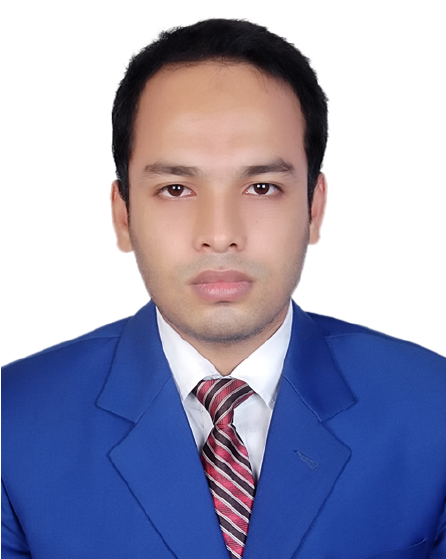
\includegraphics[width=3.1cm]{montasim.png}}}
\end{tabular*}
%------------------------------END HEADING------------------------------------





%--------------------------------START Career Objective-------------------------
\section{~~Career Objective}
  \resumeSubHeadingListStart
  \item[]
     {Practical and versatile Software Engineer with significant experience in developing software and websites. I can handle multiple tasks daily. I use a creative approach to solve problems. I am a dependable person who is great at time management. I am always energetic and eager to learn new skills.}
  \resumeSubHeadingListEnd
  \vspace{1pt}
%--------------------------------END Career Objective---------------------------





%---------------------------START Academic Qualification------------------------
\section{~~Academic Qualification}
  %-----------B.Sc.Engg. EDUCATION-----------------
  \resumeSubHeadingListStart
    \resumeSubheading
      {Bachelor of Science in Computer Science and Engineering ((B.Sc. in CSE) }{2016 - 2021}
      {Bangladesh Army University of Science and Technology (BAUST)}{}
      \vspace{.5pt}
    
    %-----------HSC EDUCATION-----------------
    \resumeSubheading
      {Higher Secondary Certificate (HSC)}{2014 - 2016}
      {Carmichael College Rangpur}{}
      \vspace{.5pt}

    %-----------SSC EDUCATION-----------------
    \resumeSubheading
      {Secondary School Certificate (SSC)}{2006 - 2014}
      {Rangpur Zilla School}{}
    \resumeSubHeadingListEnd
    \vspace{2pt}
%---------------------------END Academic Qualification--------------------------





%------------------------------------START Thesis-------------------------------
\section{Thesis}
    \resumeSubHeadingListStart
        \resumeSubItem{Undergraduate Thesis and Project}{Hand pose estimation in single RGB image with Multiview Bootstrapping.
        \newline
        - \quad Deep Learning, OpenCV, Convolutional Neural Network (CNN), Python}
    \resumeSubHeadingListEnd
    \vspace{1pt}
%------------------------------------END Thesis---------------------------------





%---------------------------START Publications----------------------------------
\begin{comment}
\section{Publications}
\resumeSubHeadingListStart
\resumeSubItem{Book: Deep Learning on Web (Web Development, Deep Learning)}{Work in Progress book to be published by Packt Publishing in late 2019. Tech: Django, Python, AWS, GCP, Azure (November '18)}
\vspace{.5pt}

\resumeSubItem{Book: Deep Learning on Mobile Devices (Flutter App Development, Deep Learning)}{Work in Progress book to be published by Packt Publishing in late 2019. Tech: Flutter, Android, Firebase, TensorFlow, Python, Dart (December '18)}
\resumeSubHeadingListEnd
\vspace{1pt}
\end{comment}
%-----------------------------END Publications----------------------------------





%---------------------------------START Experience------------------------------
\section{Experience}
  \resumeSubHeadingListStart
    \resumeSubheading
        {Web Developer}{Crystal It and Soft, Rangpur}
		{Developed and maintained affiliate marketing website.}{2019 -  2020}
        \vspace{.5pt}

    \resumeSubheading
        {Content Writer}{Crystal It and Soft, Rangpur}
		{Wrote over 150 articles/blogs for the company's various clients.}{2019 -  2020}
		\vspace{.5pt}

    \resumeSubheading
		{Problem Solver}{\href{https://www.hackerrank.com/montasim}{hackerrank.com/montasim}}
		{Solution driven programmer.}{2018 -  Present}
  \resumeSubHeadingListEnd
  \vspace{1pt}
%---------------------------------END Experience--------------------------------





%--------------------------------START Projects---------------------------------
\section{Projects}
\resumeSubHeadingListStart
\resumeSubItem{Employee Management System}{A simple Employee Management System website. With this website a company can maintain their employees. Employee can request leave from this website. Admin can manage all employees from here. 
\newline
\hspace{10mm}
- \quad PHP, Bootstrap, MySQL}
\vspace{.5pt}

\resumeSubItem{Get Your Car}{a simple car rental website. It helps you to showcase cars, rental price, speciality and so many things that are most important. This template can be used as a car rental website. 
\newline
- \quad HTML. CSS, Tailwind CSS, Bootstrap}
\vspace{.5pt}

\resumeSubItem{myCodeOnlineBootstrap}{A simple Bootstrap website template. This template can be used as a blogging website. It has Home, About, Topics and Contact Me section.
\newline
- \quad HTML. CSS, Bootstrap}
\vspace{.5pt}

\resumeSubItem{Car Game}{A simple car game. User can move car by pressing up, down, left, right arrow key. After every successful car passing points is added. Shows high score. 
\newline
- \quad Python, PyGame}
\vspace{.5pt}

\resumeSubItem{E-HealthCare}{Simple Android application which can be used as a health care app. This is an android application. It helps you find nearby hospitals, pharmacies, and Ambulance. You also can book an ambulance.
\newline
- \quad Java, Android}
\resumeSubHeadingListEnd
\vspace{1pt}
%----------------------------------END Projects---------------------------------



%-------------------------------START Skills Summary----------------------------
\section{Skills Summary}
	\resumeSubHeadingListStart
	\resumeSubItem{Programming Languages}{C, C++, JAVA, Python, PHP, SQL}
	\resumeSubItem{Web Frameworks}{Django, Flask, PyGame, Bootstrap, Tailwind CSS}
	\resumeSubItem{Web Technologies}{PHP, HTML, CSS, XML, Markdown}
	\resumeSubItem{Content Management System (CMS)}{WordPress, Blogger}
	\resumeSubItem{Databases}{SQL Server, MySQL, SQLite}
	\resumeSubItem{Toolkits}{LaTex}
	\resumeSubItem{Version Control}{Git, GitHub}
	\resumeSubItem{Operating System}{Windows(10,8.1,7), Ubuntu(16.04-20.04), Fedora, Red Hat, Kali, Linux Mint, Android}
	\resumeSubItem{IDE Experience}{Visual Studio Code, Pycharm, Android Studio, NetBeans, IntelliJ IDEA, Pycharm, CLion, Sublime \\ \hspace{28mm} Text, CodeBlocks, Nodepad++, XAMPP}
	\resumeSubItem{Office Software}{MS Word, Excel, Powerpoint}
	\resumeSubItem{Soft Skills}{Leadership, Event Management, Writing, Time Management}
\resumeSubHeadingListEnd
\vspace{1pt}
%---------------------------------END Skills Summary----------------------------





%------------------------------START Language proficiency-----------------------
\section{Language proficiency}
	\resumeSubHeadingListStart
	\resumeSubItem{English\hspace{2mm}}{Well versed in both written and spoken English}
	\resumeSubItem{Bengli\hspace{3.6mm}}{Mother tongue}
\resumeSubHeadingListEnd
\vspace{1pt}
%------------------------------END Language proficiency-------------------------





%-----------------START Training, Participation and Certification---------------
\section{Training, Participation and Certification}
\begin{description}[font=$\bullet$]
\item {Mobile Game And Application Development For Android - at ICT Division of Bangladesh}
\vspace{-5pt}
\item {PLC Training Course - at BAUST}
\vspace{-5pt}
\item {The Complete C Programming Tutorial - at Udemy online course}
\vspace{-5pt}
\item {C++ Development Tutorial Series - The Complete Coding Guide - at Udemy online course }
\vspace{-5pt}
\item {Learn C++ Programming Mini Course - Power of Animation - at Udemy online course}
\vspace{-5pt}
\item {HTML5 Coding from Scratch - Build Your Own Website - at Udemy online course}
\vspace{-5pt}
\item {Position Elements on a Page with CSS - at Coursera online course }
\vspace{-5pt}
\item {Git + GitHub for Open Source Collaboration - at Coursera online course}
\vspace{-5pt}
\item {Use Commands and Create a Remote Git Repository - at Coursera online course}
\end{description}
\vspace{1pt}
%-------------------END Training, Participation and Certification---------------




%----------------------------START Honors and Awards----------------------------
\begin{comment}
\section{Honors and Awards}
\begin{description}[font=$\bullet$]
\item {Awarded title of Intel Software Innovator - May, 2019}
\vspace{10pt}
\item {Second Runner's Up at TCS EngiNx Engineering Project Innovation Content - September, 2018 }
\vspace{-5pt}
\item {Runner's Up at Facebook Developers Circle Hackathon - August, 2017}
\end{description}
\vspace{1pt}
\end{comment}
%----------------------------END Honors and Awards----------------------------





%--------------------------START Extra Curriculum Activities--------------------
\section{Extra Curriculum Activities}
  \resumeSubHeadingListStart
	\resumeSubheading
    {Bangladesh National Cadet Corps(BNCC)}{Mohasthan Battaliont}
    {Ex. Cadet, Second best cadet at 2 Mohastan Battaliont}{2011 - 2014}
    \vspace{.5pt}
    % \vspace{10pt}\textbf{\large{Community Experience}}
    \resumeSubheading
    {Event Organizer}{Rangpur Zilla School}
    {Organized events, conducted workshops and delivered workshops}{2012 - 2014}
\resumeSubHeadingListEnd
\vspace{1pt}
%--------------------------END Extra Curriculum Activities----------------------





%-----------------------------START Personal Information------------------------
\section{Personal Information}
    \resumeSubHeadingListStart
    \item[]
        \begin{tabular}{l l}
            \textbf{Father's Name} \hspace{33mm} : \hspace{2mm} MD. Hafizar Rahman \\
            \textbf{Mother's Name} \hspace{31.4mm} : \hspace{2mm} MST. Majida Begum \\
            \textbf{Present and Parmanent Address} \hspace{1.4mm} : \hspace{2mm} Balapara 20 Mega Watt, Rangpur Sadar, Rangpur, Bangladesh \\
            \textbf{Date of Birth} \hspace{35.1mm} : \hspace{2mm} 16 December 1998 \\
            \textbf{Nationality} \hspace{39mm} : \hspace{2mm} Bangladeshi \\
            \textbf{NID No} \hspace{44.7mm} : \hspace{2mm} 195 472 8935 \\
            \textbf{Gender} \hspace{45.9mm} : \hspace{2mm} Male \\
            \textbf{Marital Status} \hspace{33.1mm} : \hspace{2mm} Married \\
            \textbf{Religion} \hspace{44.4mm} : \hspace{2mm} Islam \\
            \textbf{Blood Group} \hspace{35.7mm} : \hspace{2mm} B+ 
        \end{tabular}
    \resumeSubHeadingListEnd
    \vspace{1pt}
%-----------------------------END Personal Information----------------------





%-------------------------------START References-----------------------------
\section{~~References}
    \resumeSubHeadingListStart
        \resumeSubheading
          {Professor Dr. Md. Mamunur Rashid}{} 
          {Dean, Faculty of Electrical and Computer Engineering (ECE)}{} 
          \hfill \break
          {Bangladesh Army University of Science and Technology (BAUST)
          \newline
          Mobile: +8801769675558, Email: hdcse@baust.edu.bd}
        
        \resumeSubheading
      {Abu Saleh Musa Miah}{} 
      {Lecturer, Computer Science and Engineering (CSE)}{} 
      \hfill \break
      {Bangladesh Army University of Science and Technology (BAUST)
      \newline
      Mobile: +8801734264899, Email: abusalehcse.ru@gmail.com}
  \resumeSubHeadingListEnd
  \vspace{1pt}
%----------------------------------END References-------------------------------




%--------------------------------START Signature-------------------------
  \resumeSubHeadingListStart
  \item[]
     \vspace{50pt}
     {\hspace{120mm} .........................................................}
     \\
     {\hspace{141mm} \textbf{Signature}}
     \\
     {\hspace{115mm} Mohammad Montasim -Al- Mamun Shuvo}
  \resumeSubHeadingListEnd
  \vspace{1pt}
%--------------------------------END Signature---------------------------





\end{document}
%-------------------------------- CV ENDS HERE ---------------------------------
